\label{sota}
\minitoc
\section{Modalités des circulations des savoirs}
De nombreux$\cdot$ses chercheur$\cdot$se$\cdot$s$\cdot$x partagent le point de vue selon lequel la notion de \og{}circulation des savoirs\fg{} constitue un champ de recherche vaste, ainsi qu'un nouveau paradigme de la connaissance depuis le début du XXI\ieme{} siècle et l'avènement du Web 2.0\footnote{Cette phase de l'évolution du Web se caractérise notamment par la transformation majeure de l'Internet en vue du développement des réseaux sociaux, des blogs et des sites participatifs, tout en permettant aux utilisateur$\cdot$trice$\cdot$s$\cdot$x de créer, partager et interagir avec du contenu Web. Nous traversons actuellement l'ère du Web 3.0 qui repose sur des technologies telles que la chaîne de blocs (angl. \textit{blockchain}), le \textit{NFT} (angl. \textit{non-fungible token}), l'intelligence artificielle, métavers et le Web sémantique \citep{varet2023nouvelles}.}  (\citealp{landais2014frederic,quet2014frederic}). Le terme en question reste toutefois assez complexe en raison de visions différentes sur la façon de le définir. Afin d'éclairer cette problématique, \citeauthor{quet2014frederic} (\citeyear{quet2014frederic}, pp.~221--222) souligne trois aspects suivants :
\begin{enumerate}
    \item \textbf{Éléments de la circulation}. Qu'est-ce qui circule ? 
    \begin{itemize}
        \item individus (savants, techniciens, traducteurs, etc.) ;
        \item objets matériels (instruments scientifiques, ouvrages etc.) :
        \item constructions symboliques (théories, concepts etc.).
    \end{itemize}  
    \item \textbf{Conceptions de la circulation et méthodes de son analyse} ;
    \begin{itemize}
        \item définition de la circulation comme \og{}traduction\fg{}, \og{}diffusion\fg{}, \og{}accès\fg{} ou \og{}succès\fg{} ;
        \item critères méthodologiques possibles pour étudier la circulation p. ex. d'une théorie : 
        \begin{itemize}
            \item circulations géographiques des principaux concepteurs qu'on lui reconnaît ;
            \item circulations et lectures des textes produits par leurs concepteurs ;
            \item usages et applications analogiques qui en sont faits dans d'autres domaines.
        \end{itemize} 
        \item enjeux d'articulation de ces différents niveaux d'observation du point de vue méthodologique et de celui de la production du texte de recherche, dans le cas des croisements de ces niveaux.
    \end{itemize}
    \item \textbf{Conceptions analytiques et normatives des savoirs}
    \begin{itemize}
        \item affaiblissement des catégories des \og{}savoirs profanes\fg{} et \og{}savoirs scientifiques\fg{}, ainsi que de l'opposition entre eux ;
        \item revalorisation des savoirs implicites et de la dimension pratique des connaissances ;
        \item glorification de la circulation comme porteuse de valeurs \textit{a priori} positives : confrontation à l'autre, hybridation, production de nouveauté, etc.
    \end{itemize}
\end{enumerate}

Dans le cadre de l'analyse de l'impact scientifique de Charcot, nous étudions \textit{in fine} la circulation de ses théories et des concepts médicaux dont il était inventeur (p. ex. \textit{SLA}) et transmetteur (p. ex. \textit{hystérie})\footnote{Comme déjà expliqué dans la partie \ref{hysterie}, Charcot n'a pas inventé ce terme, mais en réinterprété le sens.}. 
%La section \ref{concept} élabore les différentes approches pour définir plus globalement la notion des concepts historiques qui nous orienteront vers une définition des concepts médicaux en particulier. \smalltodo{pont}

\section{À partir de quel moment un concept devient-il pertinent ?}
\label{concept}

Le mot \og{}concept\fg{} est un terme générique qui renvoie à un grand nombre de théories provenant de divers domaines de pensée, sans qu'il en existe une qui soit exhaustive et universellement acceptée. D'après \citeauthor{Lecourt1999} (\citeyear{Lecourt1999}, p. 224), l'invention de l'entité du concept remonte à l'ère d'Aristote, qui l'a caractérisé comme une abstraction, un mode de connaissance à la fois médiat et général, et comme mode de classification entre le genre et l'espèce (\textit{intension} et \textit{extension}). En revanche, selon les linguistes, un concept a une structure double, constituée du sens linguistique et culturel.
%dont linguistique (générale, cognitive, psycholinguistique, ethnolinguistique), philosophie, métaphysique ou mathématiques
Sa couche intérieure est constituée du noyau étymologique sur lequel repose ensuite la couche périphérique qui hérite les éléments formés par la culture, les traditions et les expériences humaines
%\foreignlanguage{russian}{(Степанов, \citeyear{stepanov2007}}). 
\footnote{En linguoculturologie, on retrouve le terme \og{}concept linguo-culturel\fg{} qui reflète cette nature double du concept.}. Il peut être exprimé par de différentes éléments du langage, soit : lexèmes, idiomes, collocations, phrases ou textes entiers \citep[p.~5]{nemickiene2011concept}. Dans le domaine du traitement automatique des langues (\textsc{TAL}), le terme \og concept \fg{} peut s'apparenter à celui des \og entités nommées \fg{}, comme en témoignent les recherches sur l'extraction automatique de la terminologie biomédicale (\citealp{jolly2024exploring,navarro2023clinical}). Un concept d'un domaine de connaissance peut faire partie d'un thésaurus, liste organisée de termes contrôlés et normalisés, auquel cas le concept est appelé \og descripteur \fg{}. \citep[p.~16]{RENNESSON202015}.



Afin de pouvoir analyser les concepts médicaux liés à Charcot, il paraît important de déterminer à partir de quel moment un mot ou un groupe de mots devient un concept en sciences humaines et sociales (ci-après SHS). Du point de vue de l'histoire des concepts (allem. \textit{Begriffsgeschichte}), cette transformation survient lorsqu'un seul mot comprend toute la gamme des significations dérivées d'un contexte sociopolitique \citep[p. 258]{koselleck2011introduction}. À titre d'exemple, le concept d'un \textit{état} ne peut être interprété qu'à travers ses différents constituants, dont \textit{souveraineté territoriale, législation, fiscalité}, parmi maints d'autres. Les concepts sont donc les concentrations par défaut ambiguës d'une multitude de contenus sémantiques, uniquement interprétables et indéfinissables, par contraste avec des significations des mots qui peuvent être définies de manière exacte \citep[p. 20]{koselleck2011introduction}. 

De plus, les concepts comme \textit{histoire} ou \textit{progrès} sont caractérisés comme \og{}collectifs singuliers\fg{} qui marquent un passage du domain concret d'un individu (plusieurs \textit{histoires} et \textit{progrès} individuels) au domain abstrait et général du collectif social (une \textit{histoire} ou un \textit{progrès} général ou collectif). Ce phénomène linguistique, ainsi que la création des concepts comme \textit{industrie, usine, classe moyenne} etc., reflète un changement de paradigme dans l'organisation sociale survenu lors des révolutions politiques et industrielles \citep[p. 1]{hobsbawm2010age}. Cela traduit donc le lien fort entre l'histoire du langage et l'histoire des idées. 
%\hl{La conceptosphere est un ensemble des concepts considerés comme caractéristique d'une nation particulière.}
Cette période charnière est nommée \textit{Sattelzeit}\footnote{Trad. allem. \og{}époque de selle\fg{}.} \citep[p.~8]{koselleck2011introduction}, entre 1750 et 1830, durant laquelle les concepts historiques deviennent abstraits, singularisés, respatialisés et retemporalisés.
 
Ces considérations peuvent s'appliquer à d'autres constructs en SHS, comme \textit{travail}, \textit{intelligencija}, \textit{Ancien Régime}, \textit{avant-garde}, \textit{Occident} etc. Elles ont acquis le statut des concepts \og{}nomades\fg{} en raison de leur circulation spatio-temporelle et linguistique \citep[p. 117]{ghermani2011}. Plusieurs questionnements ont été soulevés par la même autrice à l'égard de leur émergence, notamment pour déterminer à quel moment un concept devient une entrée dans un dictionnaire des \textsc{SHS} : \og{}\textit{Pourquoi un concept fait-il son entrée dans un dictionnaire ? Au terme de quel processus ? À l'inverse, comment cette percée lexicale est-elle parfois impossible ou refusée ?}\fg{}. Les processus permettant à un concept d'obtenir le statut de scientificité sont la propagation, la bifurcation, la capture\footnote{Termes employés par \citeauthor{stengers1987d} (\citeyear{stengers1987d}, pp.~8--22), représentatrice de la conception constructiviste du savoir scientifique.}, mais aussi les pratiques scientifiques conduisant aux masquages de sens (p. ex. dans le cas du terme \og{}confession [religieuse]\fg{}, dont le sens varie en fonction du pays dans lequel il est utilisé). 

Comme nous avons pu voir, l'histoire des concepts concerne principalement les manifestations de conflits sociopolitiques particuliers qui doivent être compris dans leur contexte approprié (p. ex. les mots comme \textit{liberté} ou \textit{démocratie} portent la connotation polémique dont le sens ne peut être précisé qu'à travers leurs antithèses). Toutefois, nous considérons que cette théorie pourrait nous permettre de formaliser une approche pour tracer l'évolution des concepts médicaux. Dans cette optique, ces concepts auront le rôle des vecteurs de la crise conceptuelle, ce qui représenterait une forme de \textit{Sattelzeit} dans le domaine de la médecine : autrement dit, ces concepts sont détournés de leurs sens initiaux neutres (descriptions des pathologies) vers ceux exerçant un certain impact sur la communauté scientifique. 






\section{Études numériques des circulations culturelles}
Incontestablement, l'époque actuelle est profondément marquée par le \og{}déluge des données\fg{}, phénomène représentatif de la quatrième paradigme de la science, selon Jim Gray \citep[p.~30]{hey2009jim}. Par conséquent, les projets numériques sont aujourd'hui \og{}pilotés par les données\fg{}\footnote{Traduction du terme \textit{data-driven} introduit par \citet{Johns1991ShouldYB}, issu de l'expression \textit{data-driven learning}.} et ceux qui sont centrés sur les explorations des circulations culturelles au prisme du numérique se concrétisent à grande échelle.
%Les humanités numériques au service de l'analyse des circulations culturelles se manifestent sous forme de divers projets de recherche au niveau académique. 
Sont fortement axés sur cette thématique :
\begin{enumerate}
\item certaines chaires universitaires, notamment celle des Humanités numériques à l'université de Genève \citep{joyeux2022circulations}\footnote{\textit{Cf.} les projets de la chaire : \url{https://www.unige.ch/lettres/humanites-numeriques/recherche/projets-de-la-chaire}.} ;
\item de divers évènements scientifiques, comme la journée d'étude \og{}Circulation des écrits littéraires de la première modernité et humanités numériques\fg{}\footnote{\url{https://www.fabula.org/actualites/86846/circulation-des-ecrits-litteraires-de-la-premiere-modernite-et-humanites-numeriques.html}}, les colloques Humanistica 2023\footnote{\url{https://humanistica2023.sciencesconf.org/}}, \textsc{ACFAS} 2023\footnote{\url{https://www.crihn.org/nouvelles/2022/12/11/colloque-de-la-transformation-des-sciences-humaines-par-les-humanites-numeriques-acfas-2023/}} etc. ;
\item des numéros de certaines revues, par exemple \og{}Circulation des discours dans les récits complotistes\fg{}, dont les articles portent sur les thématiques aussi diverses que les circulations textuelles internationales du discours complotiste des \og Illuminati \fg{}  \citep{chaudet2022illuminati}, \og conspirationniste \fg{} sur Twitter \citep{giry2022etudier} ou antiféministe en ligne \citep{morin2022discours}. 
\end{enumerate}

%Ce mémoire est basé sur la contribution de \citet{petkovic2023circulation} s'inscrivant dans l'optique de l'exploration des circulations médicales. Nous souhaitons mesurer informatiquement l'impact scientifique des travaux de Charcot sur ses collaborateurs et successeurs, membres de son réseau scientifique. Cette mesure se fonde sur l'analyse des concepts-clés en matière de son discours scientifique, et plus particulièrement sur l'opérationnalisation du terme \og{}influence\fg{}, définie ici comme une intertextualité\footnote{Nous nous appuyons sur la définition de l'intertextualité dans la littérature, où ce terme désigne \og{}la perception, par le lecteur, de rapports entre une \oe{}uvre et d'autres, qui l'ont précédée ou suivie\fg{} \citep[p.~4]{riffaterre1980trace}.} uni-directionnelle, allant des écrits de Charcot (ci-après corpus \og{}Charcot\fg{}) vers ceux de ses collaborateurs et successeurs (ci-après corpus \og{}Autres\fg{}). Il s'agit donc \textit{in fine} d'aborder computationnellement la question des circulations, non pas des artefacts matériels comme les manuscrits \citep{gabay2021katabase} et les images \citep{joyeux2019visual}, mais des phénomènes textuels complexes \citep{manjavacas} ayant une dimension théorique forte. 

La question de recherche sous-tendant ce mémoire s'approche tangentiellement des travaux de \citet{riguet2018impact} et de \citet{roe2023enlightenment}. Le premier travail porte sur la réception de la pensée scientifique du physiologiste français Claude Bernard dans la critique littéraire, illustrée par l'alignement des textes de Bernard avec des ouvrages de critique littéraire. Le second article porte sur la détection de réemplois textuels à grande échelle et l'analyse de réseaux pour identifier les \og{}influenceurs\fg{} dans les ouvrages français du siècle des Lumières.

Pour ce qui est des projets individuels, la question de l'estimation de l'importance d'une entité issue d'un domaine ontologique occupe une place centrale dans le travail de \citet{soulet2024}, ce qui a résulté dans le développement de l'outil de représentation des connaissances Rankingdom\footnote{\url{https://rankingdom.org/about}.}. L'un de ses aspects concerne les déclinaisons de la notion d'importance d'une entité, chacune correspondant à une métrique, comme présenté dans le tableau \ref{tab:rankingdom}.


\begin{table}[!h]
\centering
\footnotesize
\resizebox{\textwidth}{!}{ % Resize the table to fit within text width
\begin{tabular}{|c|c|c|}
\hline
 \rowcolor{maroon!10}
\begin{tabular}[c]{@{}c@{}}\textit{Métrique}\end{tabular} & \begin{tabular}[c]{@{}c@{}}\textit{Définition}\end{tabular}                                                                                         & \begin{tabular}[c]{@{}c@{}}\textit{Exemple}\end{tabular}                                                                                                                                             \\
\hline
\begin{tabular}[c]{@{}c@{}}\textsc{Portée}\\ (\textsc{Popularité})\end{tabular} & \begin{tabular}[c]{@{}l@{}}nombre d'assertions décrivant une entité\end{tabular}                                                                                         & Charcot est décrit par 546 assertions.                                                                                                                                                \\
\hline
\textsc{Influence}                                                     & \begin{tabular}[c]{@{}l@{}}nombre d'entités liées à une entité\end{tabular}                                                                                        & 191 entités liées à Charcot.                                                                                                                                                     \\
\hline
\textsc{À propos}                                                      & \begin{tabular}[c]{@{}l@{}}nombre d'entités impactées \\ (\oe{}uvres originales, évènements$\dots$)\end{tabular}                                                                    & 56 entités à propos de Charcot.                                                                                                                                                  \\
\hline
\textsc{Index \textit{a}}                                                       & \begin{tabular}[c]{@{}c@{}}nombre maximum d'entités impactées \textit{a} \\
ayant le comptage \og{} à propos \fg{}\end{tabular} & \begin{tabular}[c]{@{}c@{}}13 entités impactées par Charcot ont \\ le comptage \og{} à propos \fg{} supérieur à 13.\end{tabular} \\
\hline
\textsc{Impact}                                                        & \begin{tabular}[c]{@{}c@{}}somme de tous les comptages \og{} à propos \fg{}\\
de toutes les entités impactées\end{tabular}               & L'impact de Charcot est 826.                                                                                                                                                         \\
\hline
\end{tabular}
}
\caption{Aperçu des métriques Rankingdom pour quantifier l'importance d'une entité.}
\label{tab:rankingdom}
\end{table}
\bigskip
De plus, des calculs effectués à partir de la portée et de l'influence de Charcot permettent de générer un graphique de \og{}quadrant magique de Gartner\fg{} (angl. \textit{Gartner Magic Quadrant})\footnote{Le nom provient de la société américaine de conseil Gartner qui \og{}publie chaque année les résultats de ses analyses dans plus de 100 secteurs technologiques\fg{} \citep{gartner}.}. Cette représentation sur la figure \ref{fig:analyse_quadrant} met en valeur quatre types d'entités : 
\begin{itemize}
\item \textbf{acteurs de niche} : entités avec une portée et une influence modestes (p. ex. Pierre Marie) ;
\item \textit{\textbf{challengers}} : entités ayant une certaine reconnaissance et une influence considérable, mais qui sont de taille mineure, more concentrées, avec une portée plus petite (Charles-Joseph Bouchard) ;
\item \textbf{visionnaires} : entités avec une grande portée, dont l'influence reste néanmoins limitée et qui recevront plus de reconnaissance ultérieurement (Paul Richer) ;
\item \textit{\textbf{leaders}} : entités les plus importantes, avec une grande portée, connues à grande échelle et dans plusieurs domaines, tout en étant reconnues comme ayant une grande influence (Charcot).
\end{itemize}

\begin{figure}[!ht]
    \centering
    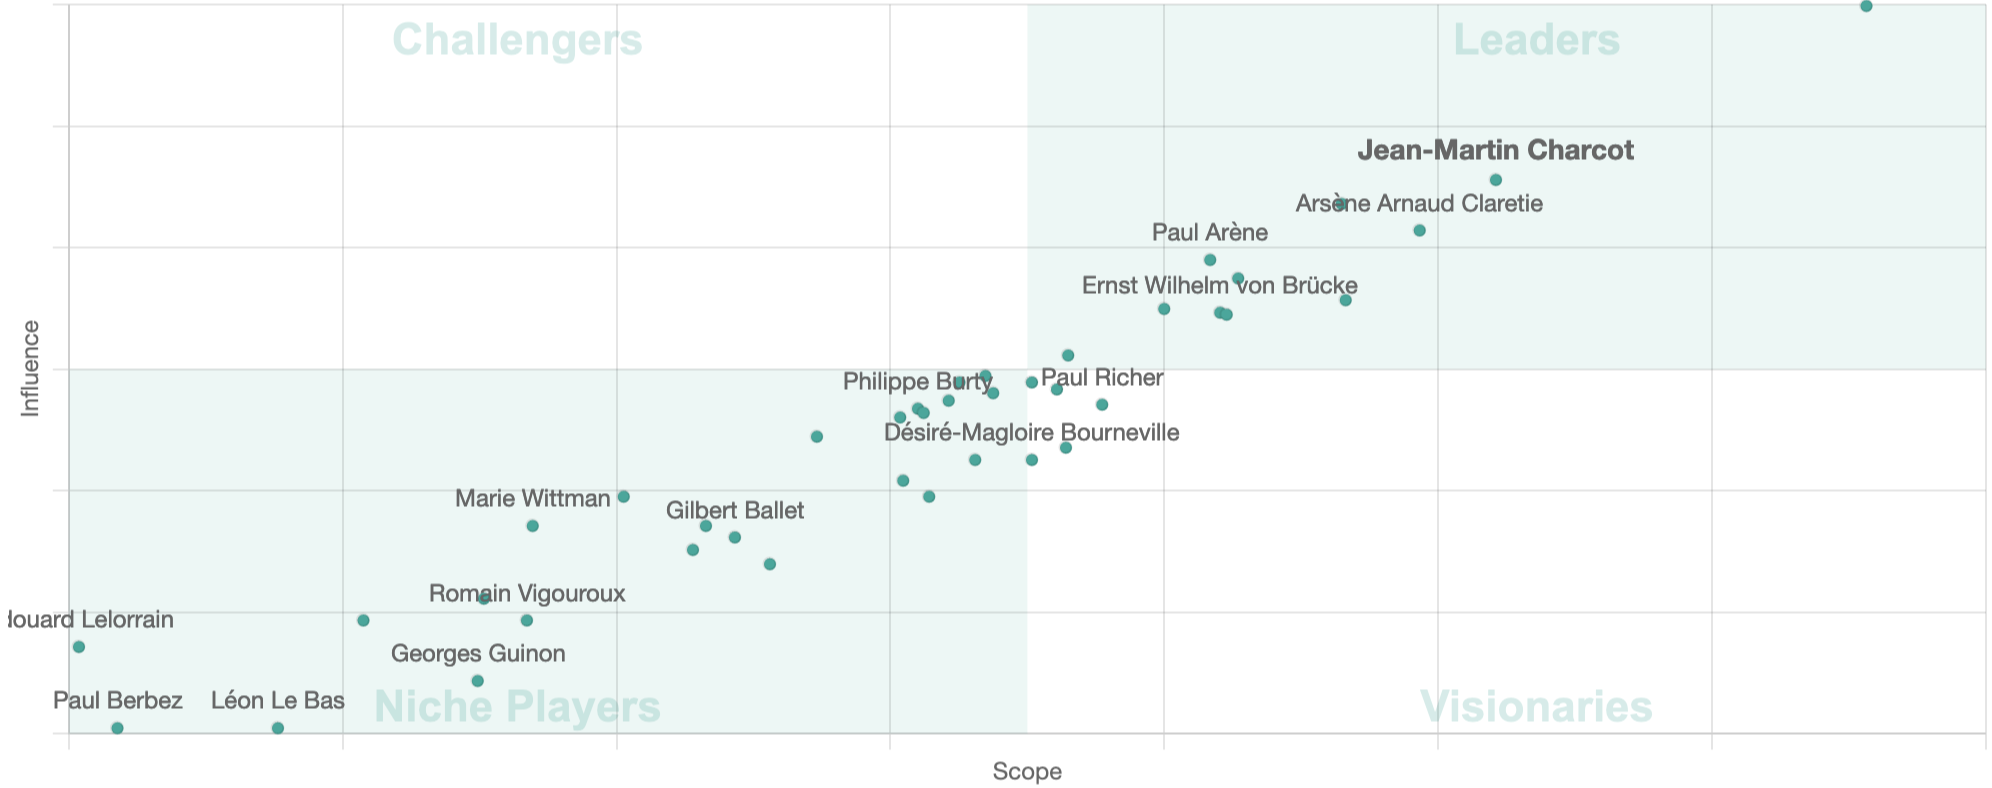
\includegraphics[width=1\textwidth]{img/analyse_quadrant.png}
    \caption[Caption for LOF]{Positionnement de l'entité \texttt{Jean-Martin Charcot} au sein de son domaine et comparaison avec les entités les plus similaires à lui \textit{via} une analyse de quadrant de l'outil Rankingdom\protect\footnotemark{.}}
    % Pour raison de visibilité, l'image originale a été agrandie, ce qui a entraîné le rapprochement des années sur l'axe de l'abscisse.
    \label{fig:analyse_quadrant}
\end{figure}

\footnotetext{\url{https://www.rankingdom.org/entity/Q20710?search=jean-martin+charcot}.}
\hl{desc brève des points principaux de cet outil : temporal analysis}

%Les humanités numériques au service de l'analyse des circulations culturelles
%
%Comment définir une circulation du point de vue de l'analyse du texte ? de la linguistique computationnelle (TAL) ?
